
\begin{figure}[p]\centering
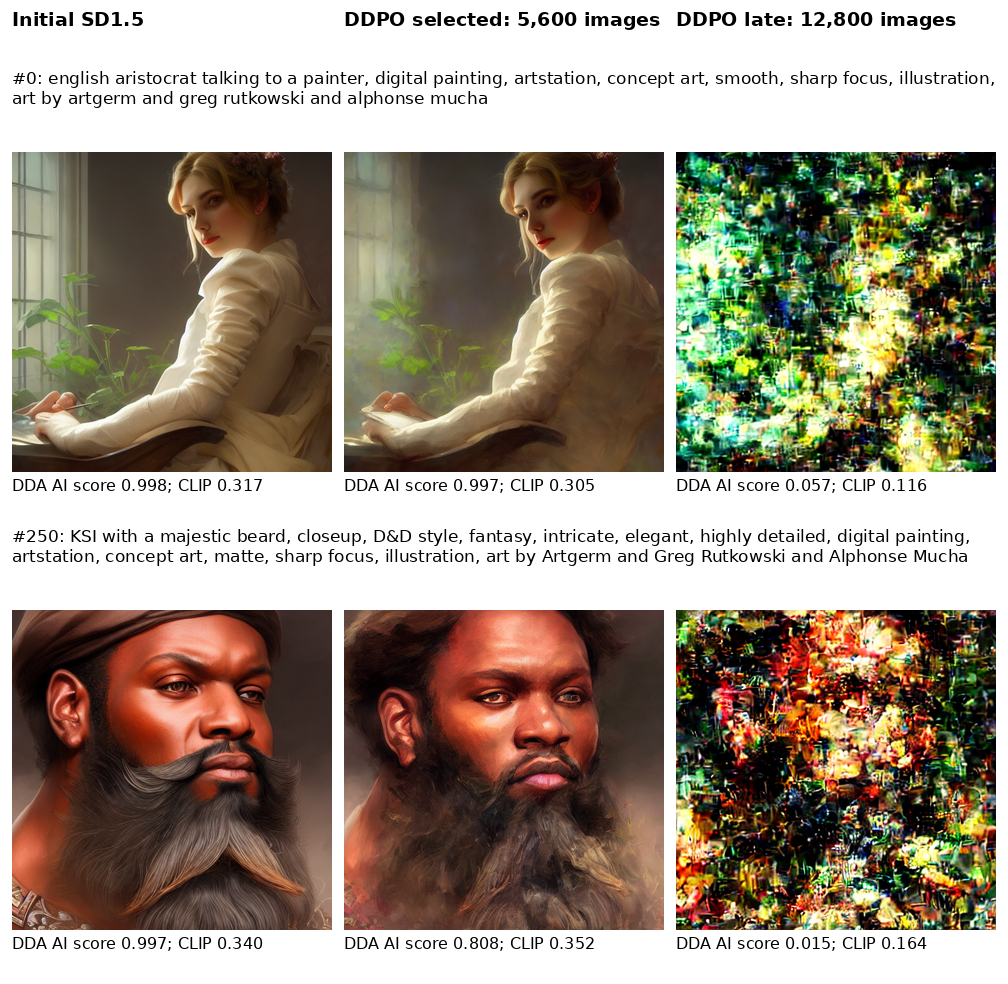
\includegraphics[width=\linewidth,height=.75\textheight,keepaspectratio]{figures/detector-sd15-comparison.png}
\caption{AI-detector evasion with unwatermarked Stable Diffusion 1.5 against the fixed, warmed DDA image classifier. Left is initial SD1.5, middle the validation-selected DDPO checkpoint after 5,600 training images, and right the later 12,800-image checkpoint evaluated exploratorily. Rows are fixed held-out positions 0 and 250 from the 500-prompt test cohort, with complete prompts shown above each row. All columns use identical prompts and DDIM sampling settings, with coupled noise seeds 20261025 plus the batch offset, 50 steps and classifier-free guidance 7.5. DDA AI scores below 0.5 count as evasion; the listed CLIP values measure prompt alignment. Selection is independent of these rows' outcomes. Uniform display resizing leaves the native 512-pixel sources unchanged.}
\label{fig:detector-image-comparison}
\end{figure}
